%%%%%%%%%%%%%%%%%%%%%%%%%%%%%%%%%%%%%%%%%%%%%%%%%%%%%
%                                                   %
%     Penn State Colloquium Poster Template         %
%                                                   %
% Uses Penn State Colloquium class, with options:   %
%                                                   %
% Orientation:                                      %
%     portrait (default), landscape                 %
%                                                   %
% Paper size:                                       %
%     a4paper (default), a0paper, a1paper, a2paper, %
%     a3paper, a5paper, a6paper                     %
%%%%%%%%%%%%%%%%%%%%%%%%%%%%%%%%%%%%%%%%%%%%%%%%%%%%%
\documentclass{../psuposter}
\renewcommand{\templateimagepath}{../} 


%%%%%%%%%%%%%%%%%%%%%%%%%%%%%%%%%%%%%%%%%%%%%%%%%%%%%
%               Package Dependencies                %
%%%%%%%%%%%%%%%%%%%%%%%%%%%%%%%%%%%%%%%%%%%%%%%%%%%%%
\usepackage{natbib}
\usepackage{lipsum}                                % Dummy text
\usepackage[figwidth = 0.98\linewidth]{todonotes}  % Dummy image (and more!)
\usepackage[absolute, overlay]{textpos}            % Figure placement
\usepackage{braket}
\setlength{\TPHorizModule}{\paperwidth}
\setlength{\TPVertModule}{\paperheight}
\setcitestyle{numbers,square}


%%%%%%%%%%%%%%%%%%%%%%%%%%%%%%%%%%%%%%%%%%%%%%%%%%%%%
%                 AUTHOR AND TITLE                  %
%%%%%%%%%%%%%%%%%%%%%%%%%%%%%%%%%%%%%%%%%%%%%%%%%%%%%
\title{Doing “Statistical Mechanics” with Big Data}
\author{Andrea Liu}
\institute{University of Pennsylvania}


%%%%%%%%%%%%%%%%%%%%%%%%%%%%%%%%%%%%%%%%%%%%%%%%%%%%%
%                  BEGIN DOCUMENT                   %
%%%%%%%%%%%%%%%%%%%%%%%%%%%%%%%%%%%%%%%%%%%%%%%%%%%%%
\begin{document}
\begin{frame}
\begin{columns}[t, totalwidth=\textwidth]
\begin{column}{0.45\textwidth - 1cm}


%%%%%%%%%%%%%%%%%%%%%%%%%%%%%%%%%%%%%%%%%%%%%%%%%%%%%
%                 BLOCK: BIOGRAPHY                  %
%%%%%%%%%%%%%%%%%%%%%%%%%%%%%%%%%%%%%%%%%%%%%%%%%%%%%
    \begin{block}{Speaker Biographic Summary}
    	\begin{center}
    		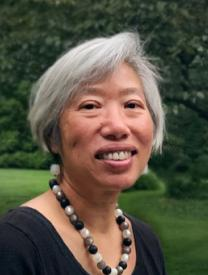
\includegraphics[width=0.55\textwidth]{images/portrait}
    	\end{center}
    	\href{https://www.physics.upenn.edu/people/standing-faculty/andrea-liu}{Prof. Andrea Liu} is a theoretical soft condensed matter physicist. She is best known for developing the field of jamming, which provides a unifying conceptual framework for understanding commonalities in systems ranging from atomic and molecular glasses, to colloidal glasses and granular matter. 
    	She received her AB degree in physics at the UC Berkeley, and her PhD in critical phenomena from Cornell in 1989. 
%    	After switching to complex fluids during her postdoc at Exxon Research and Engineering Co., she worked on polymer theory as a postdoc in the Chemical Engineering, Materials Science and Physics departments at the University of California, Santa Barbara. 
%    	She subsequently worked at Exxon Research, UCSB, and UCLA, before moving to the Department of Physics and Astronomy at the University of Pennsylvania in 2004, where she is now the Hepburn Professor of Physics. 
    	Liu is currently Past Speaker of the Council of the American Physical Society (APS) and Past Chair of the Physics Section of the American Association for the Advancement of Science (AAAS). 
    	She is a fellow of the APS, AAAS and the American Academy of Arts and Sciences, and a member of the National Academy of Sciences.
    \end{block}


%%%%%%%%%%%%%%%%%%%%%%%%%%%%%%%%%%%%%%%%%%%%%%%%%%%%%
%            BLOCK: RESEARCH INTERESTS              %
%%%%%%%%%%%%%%%%%%%%%%%%%%%%%%%%%%%%%%%%%%%%%%%%%%%%%
    \begin{block}{Research Interests}
        Prof. Liu’s research combines theory and computation to study soft and living matter. 
        In living matter, her research focuses on the role of mechanics in biology, with the aim of understanding how new and general collective phenomena. %, often beyond those typically observed in inanimate soft matter, can emerge at the subcellular, cellular and tissue levels. 
        In soft matter, she and her collaborators have shown that jamming produces solids at an opposite pole from perfect crystals, providing a new way of thinking about the nature of rigidity in disordered solids. 
%        The nonequilibrium jamming transition and jammed state thus serve as useful starting points for understanding a broad class of materials, including glasses. 
        \begin{center}
	    	
\includegraphics[width=0.65\textwidth]{images/research}    		


    	\textit{Snapshot configurations of particles identified as soft by the SVM. \cite{cubukIdentifyingStructuralFlow2015}} 
    	\end{center}

    	%\cite{longResearchLongLab}
    	
%    	Additional summary
    \end{block}
\end{column}
\begin{column}{0.55\textwidth - 1cm}


%%%%%%%%%%%%%%%%%%%%%%%%%%%%%%%%%%%%%%%%%%%%%%%%%%%%%
%                 BLOCK: ABSTRACT                   %
%%%%%%%%%%%%%%%%%%%%%%%%%%%%%%%%%%%%%%%%%%%%%%%%%%%%%
    \begin{block}{Talk Abstract}
    	Statistical mechanics has been the workhorse that condensed matter physicists have used to make the connection between microscopic properties and macroscopic, collective phenomena. Establishing this connection requires reducing masses of microscopic information (dimensional reduction) to a few relevant microscopic variables and their distributions. Data science methods are designed for dimensional reduction, so they are a natural tool to turn to when statistical mechanics fails. But it requires physics to identify the relevant microscopic quantities as well as the most appropriate data science methods to use to access them. I will discuss two problems where we have made progress with this approach: we have applied machine learning to glassy dynamics and persistent homology to the phenomenon of allostery. 
    \end{block}


%%%%%%%%%%%%%%%%%%%%%%%%%%%%%%%%%%%%%%%%%%%%%%%%%%%%%
%                BLOCK: BACKGROUND                  %
%%%%%%%%%%%%%%%%%%%%%%%%%%%%%%%%%%%%%%%%%%%%%%%%%%%%%
    \begin{block}{Brief Background}
In condensed matter physics we are often interested in gaining a microscopic understanding of macroscopic phenomena in many body systems which requires reducing microscopic information like position and velocities to averages or variances of the relevant microscopic quantities. Statistical mechanics achieves this by reducing the dimensionality of the problem to distributions of the relevant microscopic quantity at equilibrium. But in systems like glass, that form when liquids undergo transition if cooled quickly, particles remain disordered, and the relaxation time increases continuously. The time scales for equilibration become unreasonable and these systems remain far from equilibrium where ordinary statistical mechanics fails. Data science methods are designed for dimensional reduction, so they are a natural tool to turn to when statistical mechanics fails. But it requires physics to identify the relevant microscopic quantities as well as the most appropriate data science methods to use to access them. Prof. Liu's group have used Data Science methods to model such problems and consequently extract information about them for instance, the dependence of relaxation time on temperature. \cite{schoenholzStructuralApproachRelaxation2016,cubukIdentifyingStructuralFlow2015}
   	%\cite{longLocalAxonalConduction2020} 
        \begin{center}
		   	
\includegraphics[width=1\textwidth]{images/background}    	
		   	

		\textit{Phase diagrams for the dynamical loss function. \cite{ruiz-garciaTiltingPlayingField2021}}	
    	\end{center}
%		Second Paragraph 
		%\cite{longMorphologicalCharacterizationHVC2018} 
    \end{block}


%%%%%%%%%%%%%%%%%%%%%%%%%%%%%%%%%%%%%%%%%%%%%%%%%%%%%
%                 BLOCK: REFERENCES                 %
%%%%%%%%%%%%%%%%%%%%%%%%%%%%%%%%%%%%%%%%%%%%%%%%%%%%%
    \begin{block}{References}
    	\nocite{*}
        \bibliographystyle{aipnum4-1}
%        \bibliographystyle{iopart-num}
		\bibliography{references}
    \end{block}

\end{column}
\end{columns}


%%%%%%%%%%%%%%%%%%%%%%%%%%%%%%%%%%%%%%%%%%%%%%%%%%%%%
%                    FOOTER TEXT                    %
%%%%%%%%%%%%%%%%%%%%%%%%%%%%%%%%%%%%%%%%%%%%%%%%%%%%%
\begin{textblock}{0.5}(0.18, 0.94)
    \color{white}
    \sffamily
    \textbf{Eberly College of Science}
    \\
    Department of Physics
\end{textblock}


%%%%%%%%%%%%%%%%%%%%%%%%%%%%%%%%%%%%%%%%%%%%%%%%%%%%%
%                   END TEMPLATE                    %
%%%%%%%%%%%%%%%%%%%%%%%%%%%%%%%%%%%%%%%%%%%%%%%%%%%%%
\end{frame}
\end{document}
